% file: math/full-binary-tree.tex

\documentclass{standalone}
\usepackage{tikz}
\usepackage{tikz-qtree}

\begin{document}

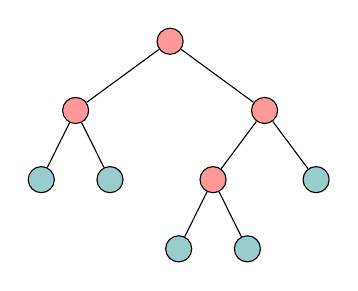
\begin{tikzpicture}[level distance = 25pt, sibling distance = 15pt,
  edge from parent/.style= {
      draw, edge from parent path = {(\tikzparentnode) -- (\tikzchildnode)}}]
  \tikzset{every tree node/.style = {align = center, circle, draw, fill = red!40},
      leaf/.style = {fill = teal!40}}

    \Tree [.{}  [.{} [.\node[leaf](l1){}; ]
		     [.\node[leaf](l2){}; ]
                ]
		[.{} 
		  [.{} 
		    [.\node[leaf](l3){}; ] 
		    [.\node[leaf](l4){}; ]
		  ] 
		  [.\node[leaf](l5){}; ]
		] 
	  ]
\end{tikzpicture}
\end{document}